\documentclass[../../../../main.tex]{subfiles}
\begin{document}

$\ell$ を座標平面上の原点を通り傾きが正の直線とする。
さらに，以下の3条件 (i)，(ii)，(iii) で定まる円 $C_1$，$C_2$ を考える。

\begin{enumerate}
  \item 円 $C_1$，$C_2$ は2つの不等式 $x\geqq0$，$y\geqq0$ で定まる領域に含まれる。
  \item 円 $C_1$，$C_2$ は直線 $\ell$ と同一点で接する。
  \item 円 $C_1$ は $x$ 軸と点 $(1, \, 0)$ で接し，円 $C_2$ は $y$ 軸と接する。
\end{enumerate}

円 $C_1$ の半径を $r_1$，円 $C_2$ の半径を $r_2$ とする。
$8r_1+9r_2$ が最小となるような直線 $\ell$ の方程式と，その最小値を求めよ。

\begin{figure}[htbp]
  \centering
  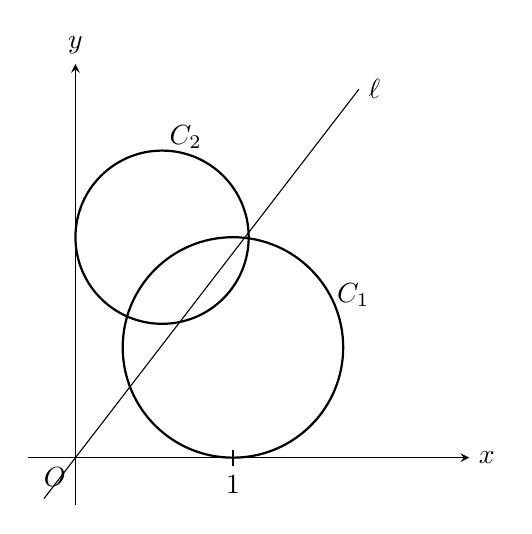
\begin{tikzpicture}[scale=2, >=stealth]
    \draw[->] (-0.3,0) -- (2.5,0) node[right] {$x$};
    \draw[->] (0,-0.3) -- (0,2.5) node[above] {$y$};
    \node[below left] at (0,0) {$O$};

    \draw (-0.2, -0.26) -- (1.8, 2.34) node[right] {$\ell$};

    \draw[thick] (1, 0.7) circle (0.7);
    \node[above right] at (1.6, 0.9) {$C_1$};
    \draw (1, 0.05) -- (1, -0.05) node[below] {$1$};

    \draw[thick] (0.55, 1.4) circle (0.55);
    \node[above] at (0.7, 1.9) {$C_2$};
  \end{tikzpicture}
\end{figure}

\end{document}
